\documentclass[12pt]{beamer}
\usepackage[T2A]{fontenc}
\usepackage[utf8]{inputenc}
\usepackage[english]{babel}
\usepackage{amssymb,amsfonts,amsmath,mathtext}
\usepackage{cite,enumerate,float,indentfirst}
\usepackage{longtable,xspace,subcaption}  
% \usepackage{euler}
\usepackage{amsmath}

\graphicspath{{images/}}

\usetheme{Singapore}
\usecolortheme{beaver}

\setbeamercolor{footline}{fg=red}
\setbeamertemplate{footline}{
  \leavevmode%
  \hbox{%
  \begin{beamercolorbox}[wd=.333333\paperwidth,ht=2.25ex,dp=1ex,center]{}%
    Innopolis University
  \end{beamercolorbox}%
  \begin{beamercolorbox}[wd=.333333\paperwidth,ht=2.25ex,dp=1ex,center]{}%
    CloSpan
  \end{beamercolorbox}%
  \begin{beamercolorbox}[wd=.333333\paperwidth,ht=2.25ex,dp=1ex,right]{}%
  page \insertframenumber{} of \inserttotalframenumber \hspace*{2ex}
  \end{beamercolorbox}}%
  \vskip0pt%
}
\fontsize{9}{10}\selectfont
\newcommand\fontvi{\fontsize{10}{12}\selectfont}
\newcommand{\itemi}{\item[\checkmark]}
\title{\fontsize{15}{15}\selectfont
	\textbf{Mining Closed Sequential Patterns in Large Datasets
}}
\author{
	\fontvi
	\small{%	
\emph{Presenter:}~Ildar Nurgaliev\\%
\emph{Lab:}~Dainfos}\\%
}
\titlegraphic{
\includegraphics[width=0.2\linewidth]{iu}}
\date{}

\begin{document}

\maketitle

\begin{frame}{Main idea}
  Instead of mining the complete set of frequent subsequences we mine frequent \textit{closed subsequences}
\end{frame}

\begin{frame}{Benefits}
\begin{itemize}
\item can mine really long sequences
\item produce significantly less number of discovered frequent sequences
\end{itemize}
\end{frame}

\begin{frame}{Preliminary Concepts}{Sequence}
\begin{itemize}
\item items: $\textit{I} = \{i_1, i_2, ..., i_m\}$
\item itemset ($t_i$): $t_i \subseteq \textit{I}$
\item sequence (ordered list): $s = \langle t_1, t_2, ..., t_m \rangle$
\item size |s|: number of itemsets in s
\item length l(s): $l(s)=\sum\limits_{i=1}^n |t_i|$
\end{itemize}
\end{frame}

\begin{frame}{Preliminary Concepts}{$\alpha$ sub-sequence of $\beta$ OR $\beta$ super-sequence of $\alpha$ (contains)}
\begin{itemize}
\item $\alpha = \langle \alpha_1, \alpha_2, ..., \alpha_m \rangle$
\item $\beta = \langle \beta_1, \beta_2, ..., \beta_m \rangle$
\item $\alpha \sqsubseteq \beta$ (if $\alpha \neq \beta$, written as $\alpha \sqsubset \beta$)
\item iff $\exists i_1, i_2,...,i_m$, such that\\ $1 \leq i_1 \textless i_2 \textless ... \textless i_m \leq n$ and\\ $\alpha_1 \subseteq \beta_i,\alpha_2 \subseteq \beta_{i_2},...,\alpha_m \subseteq \beta_{i_m}$
\item $\beta$ absorbs $\alpha$: if $\beta$ contains $\alpha$ and their \textit{support} are the same
\end{itemize}
\end{frame}

\begin{frame}{Preliminary Concepts}{Support}
\begin{itemize}
\item $\textit{D} = \{ s_1,s_2,...,s_n \}$: sequence database
\item each \textit{s} associated with \textit{id} (id of $s_i$ is \textit{i})
\item |$\textit{D}$|: number of \textit{s} in \textit{D}
\item $support(\alpha)$: number of \textit{s} in \textit{D} which contain $\alpha$\\
$support(\alpha) = |\{ s|s \in D~and~\alpha \sqsubseteq s\}|$
\item \textit{min\_sup}: minimum support threshold
\end{itemize}
\end{frame}

\begin{frame}{Preliminary Concepts}{Frequent sequential pattern (FS) and closed FS (CS)}
\begin{itemize}
\item FS: includes all s of $\textit{support(s)} \leq \textit{min\_sup}$
\item $CS = \{ \alpha|\alpha \in~FS~and~\nexists\beta \in$ FS\\such that $\alpha \sqsubseteq \beta~and~support(\alpha) = support(\beta)\}$
\item {\bf {\it closed sequence mining}}: find CS above {\it min\_sup}
\item database containment relation $D \sqsubseteq D'$:\\if $\exists$ an injective function $f : D \rightarrow D'$, s.t.\\
$\forall s \in D, s \sqsubseteq f(s)$
\end{itemize}
\end{frame}

\begin{frame}{Preliminary Concepts}{Item extension}
\begin{itemize}
\item Given: $s = \langle t_1,...,t_m \rangle$ and item $\alpha$
\item $s \diamond \alpha$: concatenation (I-Step or S-Step)
\item $s \diamond_i \alpha = \langle t_1,...,t_m \cup \{ \alpha \} \rangle$ if $\forall k \in r_m, k \textless \alpha$\\ Example: $\langle (\alpha e) \rangle$ is I-Step extension of $\langle (\alpha) \rangle$
\item $s \diamond_s \alpha = \langle t_1,...,t_m,\{ \alpha \} \rangle$\\ Example: $\langle (\alpha)(c) \rangle$ is S-Step extension of $\langle (\alpha) \rangle$
\end{itemize}
\end{frame}

\begin{frame}{Preliminary Concepts}{Sequence extension}
\begin{itemize}
\item Given: $s = \langle t_1,...,t_m \rangle$ and $p = \langle t_1',...,t_n' \rangle$
\item $s \diamond p$: concatenation (itemset-extension or sequence-extension)
\item $s \diamond_i p = \langle t_1,...,t_m \cup t_1',...,t_n' \rangle$ if $\forall k \in t_m, j \in t_1', k \textless j$
\item $s \diamond_s p = \langle t_1,...,t_m,t_1',...,t_n' \rangle$
\item $s' = p \diamond s$: p - prefix and s - suffix of $s'$\\ Example: $\langle (e)(\alpha) \rangle$ is prefix of $\langle (e)(abf)(bde) \rangle$ and $\langle (bf)(bde) \rangle$ is its suffix
\end{itemize}
\end{frame}

\begin{frame}{Preliminary Concepts}{{\it s-projected} database ({\it physical projection } and {\it pseudo projection})}
\begin{itemize}
\item $D_s = \{p | s' \in D, s' = r \diamond p$ ~~s.t. r is minimum prefix containing s ($s \sqsubseteq r$ and $\nexists r',s \sqsubseteq r' \sqsubset r$)\}\\ p can be empty
\end{itemize}
\begin{figure}
\center{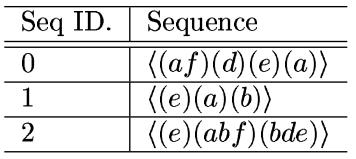
\includegraphics[width=0.4\linewidth]{D}}\caption*{Example}
\end{figure}
\begin{itemize}
\item $D_{\langle (\alpha f) \rangle} = \{ \langle (d)(e)(\alpha) \rangle, \langle (bde) \rangle \}$
\item $D_{\langle (e)(\alpha) \rangle} = \{ \$,\langle (b) \rangle,\langle (\_bf)(bde) \rangle \}$
\end{itemize}
\end{frame}

\begin{frame}{Lexicographic Sequence Tree}{{\it Set Lexicographic Order}}
\begin{itemize}
\item Let $t = \{ i_1,i_2,...,i_k\}, t'=\{j_1,j_2,...,j_l\}$, where $i_1 \leq ... \leq i_k$ and $j_1 \leq ... \leq j_l$
\item $t < t'$ iff {\it either} of the following is true:
\begin{enumerate}
\item $0 \leq h \leq min\{k,l\}$, we have $i_r = j_r$ for $r < h$, and $i_h < j_h$
\item $k < l$, and $i_1 = j_1,i_2 = j_2,...,i_k=j_k$
\end{enumerate}
\end{itemize}
Example: $(a,f) < (b,f), (a,b) < (a,b,c)$ and $(a,b,c) < (b,c)$
\end{frame}

\begin{frame}{Lexicographic Sequence Tree}{{\it Sequence Lexicographic Order}}
\begin{enumerate}[i]
\item if $s' = s \diamond p$, then $s < s'$
\item if $s = \alpha \diamond_i p$ and $s' = \alpha \diamond_s p'$, no matter what is order relation between $p$ and $p'$ is, $s < s'$
\item if $ s = \alpha \diamond_i p$ and $s' = \alpha \diamond_i p',~p < p'$ indicated $s < s'$
\item $s = \alpha \diamond_s p$ and $s' = \alpha \diamond_s p',~p < p'$ indicates $s < s'$
\end{enumerate}
Example: $\langle (a,b) \rangle < \langle (a,b)(a) \rangle$; $\langle (a,b) \rangle < \langle (a)(a) \rangle$
\end{frame}

\begin{frame}{Lexicographic Sequence Tree}{{\it Lexicographic Sequence Tree} construction}
\begin{enumerate}[i]
\item if $s' = s \diamond p$, then $s < s'$
\item if $s = \alpha \diamond_i p$ and $s' = \alpha \diamond_s p'$, no matter what is order relation between $p$ and $p'$ is, $s < s'$
\item if $ s = \alpha \diamond_i p$ and $s' = \alpha \diamond_i p',~p < p'$ indicated $s < s'$
\item $s = \alpha \diamond_s p$ and $s' = \alpha \diamond_s p',~p < p'$ indicates $s < s'$
\end{enumerate}
Example: $\langle (a,b) \rangle < \langle (a,b)(a) \rangle$; $\langle (a,b) \rangle < \langle (a)(a) \rangle$
\end{frame}

% \begin{frame}{Results}{Classification on data with 3 labels, cross-validation = 3}
% \fontsize{11}{14}\selectfont
% \begin{longtable}{| c | c | c |}
% \hline
% Classifier & Clean features & Improvement with\\ 
% & Performance & GA Performance\\
% \hline
% Gaussian Naive Bayes & 41\% (+/- 5) & 48.2\%\\
% \hline
% Logistic regression & 63\%  (+/- 2) & 66.3\% \\
% \hline
% \textbf{k-NN} & 59\% (+/- 4) & 68.6\% \\
% \hline
% 1-NN & 52\% (+/- 3) & 62\% \\
% \hline
% SVM-rbf & 62\% (+/- 9) & 66.2\% \\
% \hline
% SVM-inear & 60\% (+/- 3) & 65.5\% \\
% \hline
% \end{longtable}
% \end{frame}

\end{document}